\documentclass[a4paper, 12pt]{article}

\newcommand{\templates}{../../template}
\usepackage[a4paper, margin=2.5cm]{geometry}

\usepackage{enumitem}
\setlist[itemize]{noitemsep}
\setlist[enumerate]{noitemsep}

\let\oldpar\paragraph
\renewcommand{\paragraph}[1]{\oldpar{#1\\}\noindent}
\usepackage{graphicx}
\usepackage{hyperref}
\usepackage{makecell}

\newcommand{\settitolo}[1]{\newcommand{\titolo}{#1\\}}
\newcommand{\setprogetto}[1]{\newcommand{\progetto}{#1\\}}
\newcommand{\setcommittenti}[1]{\newcommand{\committenti}{#1\\}}
\newcommand{\setredattori}[1]{\newcommand{\redattori}{#1\\}}
\newcommand{\setrevisori}[1]{\newcommand{\revisori}{#1\\}}
\newcommand{\setresponsabili}[1]{\newcommand{\responsabili}{#1\\}}
\newcommand{\setversione}[1]{
	\ifdefined\versione\renewcommand{\versione}{#1\\}
	\else\newcommand{\versione}{#1\\}\fi
}
\newcommand{\setdestuso}[1]{\newcommand{\uso}{#1\\}}
\newcommand{\setdescrizione}[1]{\newcommand{\descrizione}{#1\\}}

\newcommand{\makefrontpage}{
	\begin{titlepage}
		\begin{center}

		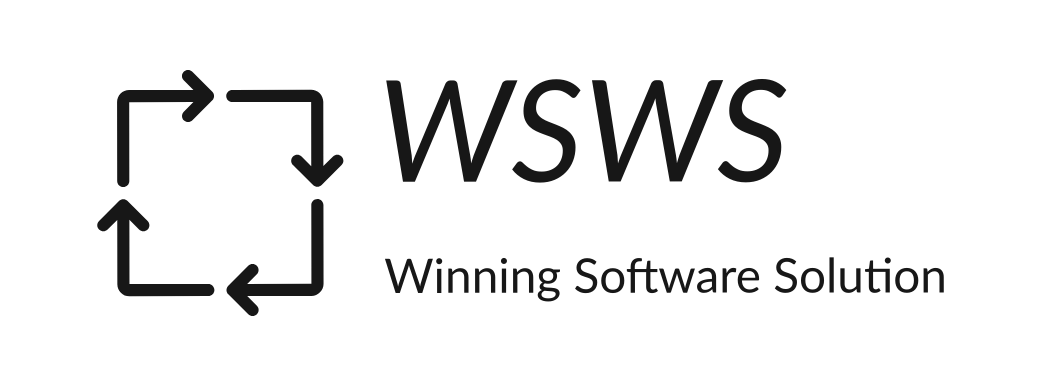
\includegraphics[width=0.4\textwidth]{../../template/WSWS-logos_transparent_crop}\\

		{\Large Winning Software Solution}\\[6pt]
		\href{mailto://winningsoftwaresolution@gmail.com}{winningsoftwaresolution@gmail.com}\\
		
		\ifdefined\progetto
		\vspace{1cm}
		{\Large\progetto}
		{\large\committenti}
		\else\fi
		
		\vspace{1.5cm}
		{\LARGE\titolo}
		
		\vfill
		
		\begin{tabular}{r | l}
		\multicolumn{2}{c}{\textit{Informazioni}}\\
		\hline
		
		\ifdefined\redattori
			\textit{Redattori} &
			\makecell[l]{\redattori}\\
		\else\fi
		\ifdefined\revisori
			\textit{Revisori} &
			\makecell[l]{\revisori}\\
		\else\fi
		\ifdefined\responsabili
			\textit{Respondabili} &
			\makecell[l]{\responsabili}\\
		\else\fi
		
		\ifdefined\versione
			\textit{Versione} & \versione
		\else\fi
		
		\textit{Uso} & \uso
		
		\end{tabular}
		
		\vspace{2cm}
		
		\ifdefined\descrizione
		Descrizione
		\vspace{6pt}
		\hrule
		\descrizione
		\else\fi
		\end{center}
	\end{titlepage}
}
\usepackage{hyperref}
\usepackage{array}
\usepackage{tabularx}

\def\vers#1-#2-#3-#4-#5\\{#1&#2&#3&#4&#5\\\hline}

\newcommand{\addversione}[5]{
	\ifdefined\versioni
		\let\old\versioni
		\renewcommand{\versioni}{#1&#2&#3&#4&#5\\\hline\old}
	\else
		\newcommand{\versioni}{#1&#2&#3&#4&#5\\\hline}
	\fi
}

\newcommand{\setversioni}[1]{\newcommand{\versioni}{#1}}

\newcommand{\makeversioni}{
	\begin{center}
		\begin{tabularx}{\textwidth}{|c|c|c|c|X|}
		\hline
		\textbf{Versione} & \textbf{Data} & \textbf{Persona} & \textbf{Attivtà} & \textbf{Descrizione} \\
		\hline
		\versioni
		\end{tabularx}
	\end{center}
	\clearpage
}

\settitolo{Analisi delle tecnologie}
\setredattori{Federico Marchi \\ Matteo Galvagni}
\setdestuso{interno}
\setdescrizione{
Analisi delle tecnologie.
}

\begin{document}

\makefrontpage

\section{Analisi delle Blockchain}

\subsection*{Premesse}
Le metriche di valutazione sono state scelte in base alla loro importanza sia nella normale valutazione di una blockchain sia nello svolgimento di questo particolare progetto.
È importante tenere in considerazione che, mentre alcune delle metriche sono dati di fatto, altre sono medie o stime teoriche che è importante approfondire prima di trarre una conclusione.
Di seguito una rapida spiegazione di ogni metrica scelta.

\subsubsection*{Scalabilità}
Gli attributi scelti per valutare la scalabilità di ogni blockchain mirano non solo a dare un'idea della velocità e dei costi attuali per operare su ogni rete, ma anche a stimare come tale
rete potrebbe performare in futuro e/o in periodi di congestione per via di un ipotetico aumento della domanda di utilizzo.

\begin{itemize}
\item \textbf{Transaction fee: }
È il costo medio \textit{attuale} per effettuare una normale transazione sulla rete.
È un costo personalizzabile: nulla vieta infatti di impostare un costo più alto del normale per assicurarsi una velocità di transazione maggiore o viceversa.
Questa metrica è fondamentale per una buona riuscita del progetto in esame, in quanto è assolutamente preferibile che al momento della scannerizzazione del codice QR
il cliente paghi una cifra insignificante (idealmente, nell'ordine dei centesimi o inferiore) per chiamare la funzione dello \textit{smart contract} che si occuperà di sbloccare i fondi
al venditore. È inoltre preferibile, ma meno significativo del precedente esempio, che anche in fase d'acquisto la tassa di transazione sia molto bassa, anche se
in questa particolare fase una tassa di poche decine di centesimi è considerata accettabile in quanto pressoché in linea con il costo della competizione (Es.: prezzo di un bonifico;
tassa percentuale trattenuta da servizi come \textit{Paypal}).
È inoltre necessario esaminare come il costo per transazione cambierebbe in caso di un aumento della domanda di utilizzo della blockchain, per garantire un funzionamento
accettabile anche nel futuro.

\item \textbf{Transaction time: }
Anche detta \textit{Transaction finality}, è il tempo medio \textit{attuale} in cui una transazione viene confermata e inserita permanentemente nella blockchain.
Esso è la somma del tempo in cui la transazione, una volta emessa, viene accettata da un miner/validatore inserendola in un blocco e il tempo impiegato da tale blocco per essere
approvato. Dipende direttamente dalla tassa di transazione: se viene impostato un costo molto più alto del normale i miners/validatori saranno incentivati a includere tale transazione
in un blocco e approvare quel blocco il prima possibile, così da aggiudicarsi la tassa di transazione. Al contrario, una tassa impostata per risultare in una transazione più economica
sarà scelta per ultima dai miners/validatori, in quanto non hanno incentivo economico ad approvare tale transazione prima di altre che pagano di più.
Per il progetto in esame è fondamentale un tempo di transazione molto basso (idealmente nell'ordine dei secondi) poichè il cliente nella fase di scannerizzazione del codice QR deve
avere un'esperienza veloce.

\item \textbf{Block time: }
È il tempo medio \textit{attuale} in cui un blocco viene approvato nella blockchain. Indica la velocità con quale i miners/validatori di una rete approvano un blocco e va valutato insieme al parametro "grandezza di blocco": un blocco molto grande può contenere molte transazioni, quindi anche con un tempo di blocco non esemplare il tempo di transazione diminuisce considerevolmente
perchè molte più transazioni possono essere incluse in un blocco, anche quelle che eventualmente rendono meno profitto ai miners/validatori; al contrario, con un blocco molto piccolo la velocità
di approvazione di un blocco perde di importanza perchè molte meno transazioni possono essere incluse in un blocco creando forte competizione per ottenere l'approvazione della transazione risultando
in transazioni con costi impostati per essere medio-bassi molto più lente.

\item \textbf{Block size: }
È il peso in memoria di un blocco. È proporzionale al numero di transazioni che un blocco può contenere: un blocco molto grande risulta in una velocità di transazione alta e un costo per transazione
moderato/basso perchè c'è poca competizione da parte delle transazioni per essere inserite nel blocco, come spiegato nel punto precedente. Di contro, un blocco molto grande richiederebbe
hardware più costoso per essere approvato nella blockchain (nel caso di reti con algoritmo di consenso PoW), creando una pressione di centralizzazione della rete verso enti con più disponibilità economica. Un blocco molto grande, indipendentemente dall'algoritmo di consenso, creerebbe la possibilità di transazioni così economiche che vi sarebbe un reale rischio di attacchi simili
al dDos (spam di transazioni) che farebbero crescere di grandezza la blockchain a dismisura, richiedendo ai nodi hardware più costoso per memorizzarla e creando una pressione verso la centralizzazione. //manca roba qua


\end{itemize}
\subsubsection*{Sicurezza \& Decentralizzazione}
Le metriche di valutazione della sicurezza e della decentralizzazione vogliono invece dare una stima teorica del livello di resistenza di ogni rete a possibili attacchi da parte di entità
malevole. I tipi di attacchi possono avere natura diversa: è necessario che la rete scelta sia protetta sia da attacchi di tipo economico (Es.: gli sviluppatori vendono una grande quantità
di token nativi nel tentativo di intascare il denaro degli investitori facendo crollare prezzo del token e la fiducia verso la rete; un'entità include una transazione malevola (spesa
di token non posseduti) in un blocco e riesce a minarlo/validarlo) sia da attacchi mirati alla distruzione della rete (Es.: uno o pochi stati vietano il mining/la validazione dei blocchi
e la rete perde gran parte o la totalità dei suoi nodi; un'azienda che controlla gran parte dei miners/validatori chiude o viene a sua volta attaccata e l'intera rete va offline).

\subsection*{Ethereum}
\subsection*{Polygon}
\subsection*{xDai}
\subsection*{Solana}
\subsection*{Algorand}
\subsection*{Avalanche}
\subsection*{Fantom}
\subsubsection*{Scalabilità}
Si tratta di una blockchain ad alta scalabilità, infatti esegue quasi istantaneamente le transazioni a costi pressoché trascurabili.
\subsubsection*{Sicurezza \& Decentralizzazione}
L' algoritmo di consenso utilizzato si chiama Lachesis, si tratta di un PoS con BTF (Byzantine Fault Tolerance) secondo il quale la blockchain rimane stabile e in funzione fin tanto che i $\frac{2}{3}$ dei validatori non è malevolo.
Da un lato questo algoritmo potrebbe facilitare un'ipotetico attacco alla blockchain, tuttavia essendo complesso e oneroso diventare validatore risulta alla fine complesso e controproducente attaccare la blockchain.
Per poter diventare validatore sono necessari 1 milione di FTM (token nativo di Fantom), circa l’equivalente di 2 milioni di dollari.
Pecca sotto l’aspetto della decentralizzazione poiché sono presenti solo 60 validatori momentaneamente, di cui 10 appartenenti alla Fantom Foundation.
\subsubsection*{Considerazioni finali}
Nonostante sia una delle migliori blockchain sotto il punto di vista della scalabilità, non è stata scelta poiché riteniamo, al fine di garantire una lunga prospettiva di vita al progetto, che sia fondamentale utilizzare una blockchain maggiormente decentralizzata, dunque con un numero di validatori superiore.
\subsection*{Cardano}
\subsection*{Harmony}
\section{Analisi seconda tecnologia}
\end{document}
